\documentclass[ebook]{sigproc}

\directlua{if not (os.env["MODE"] == "production") then tex.sprint("\\usepackage[colorspec=0.9]{draftwatermark}") end}

\usepackage{graphicx,xcolor}
\usepackage[unicode,pdfusetitle]{hyperref}
\usepackage{xr,subfiles}
\usepackage{pdfpages}
\usepackage{makeidx}
\usepackage{comment}

% styles/ 以下のスタイルファイル
\usepackage{indexsymbol}
\usepackage{sigproc-base}
\usepackage{sigproc-math}

% メタデータ
\title{信号解析の数理}
\author{calamari\_dev}
\date{\today}

\definecolor{linkcolor}{RGB}{26,13,171}
\hypersetup{
  pdfsubject={線型代数で信号を理解するために},
  pdfkeywords={線型代数,関数解析,時間周波数解析,信号処理},
  colorlinks=true,
  allcolors=linkcolor
}

% 各種パッケージの初期設定
\externaldocument[xr-]{\subfix{main}}
\makeindex

\begin{document}

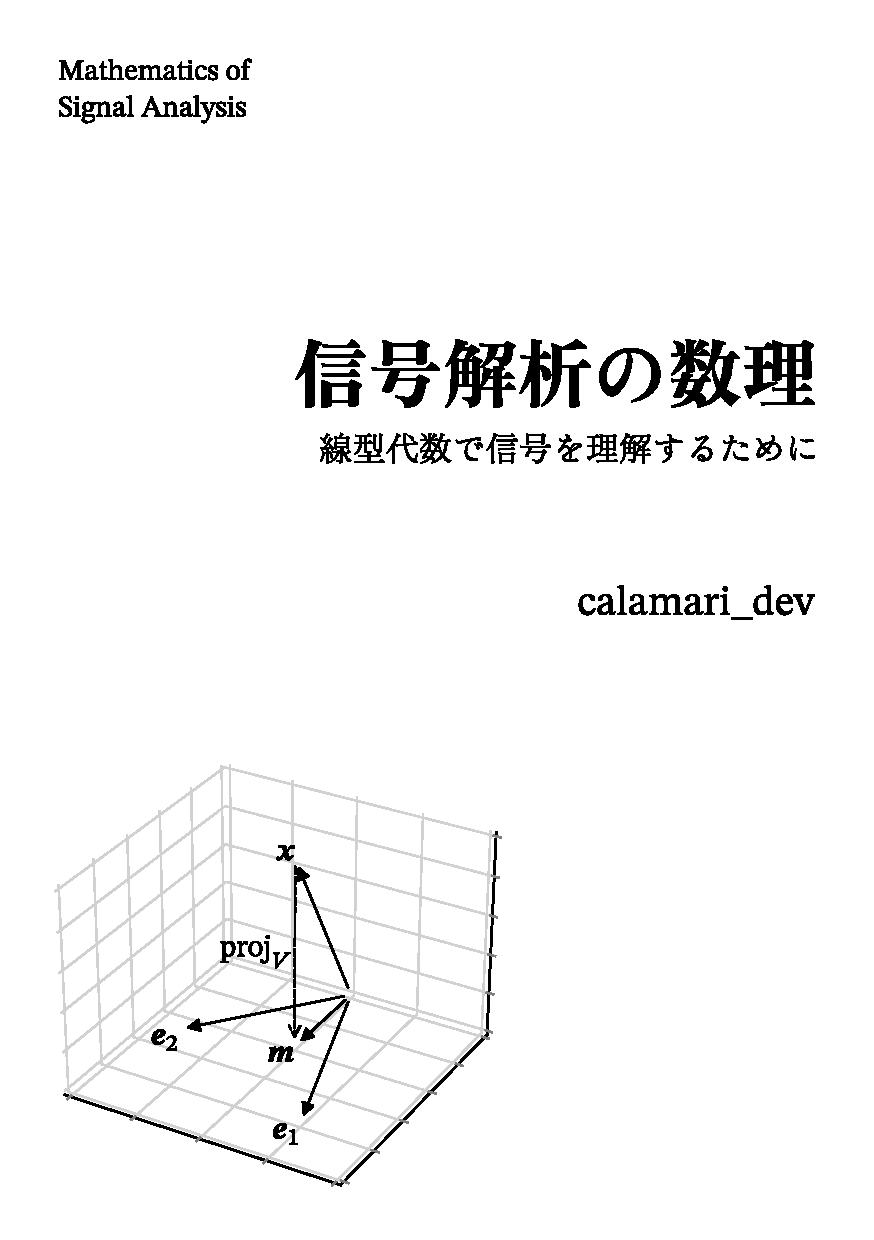
\includepdf{titlepage/titlepage.pdf}

\frontmatter

\subfile{chapter/getting_started/index}

\tableofcontents

\subfile{chapter/symbols/index}

\mainmatter

\subfile{chapter/preliminary/index}

\subfile{chapter/numerical_vector_space/index}

\subfile{chapter/hilbert_space/index}

\subfile{chapter/probability_space/index}

\appendix
\pagestyle{appendix}

\subfile{chapter/program_example/index}

\backmatter

\subfile{chapter/references/index}

\printindex

\end{document}
